%! Author = Len Washington III
%! Date = 9/11/24

% Preamble
\documentclass[
	number={4},
	title={Logistic Regression}
]{cs584notes}

% Document
\begin{document}

\section{Generative Classifiers}\label{sec:generative-classifiers}
If we are \emph{distinguishing} cat from dog images using a \emph{Generative Classifier}, we \emph{build} a \emph{model} of what is in a \emph{cat image}.
\begin{itemize}
	\item Knows about whiskers, ears, eyes.
	\item \emph{Assigns a probability} to any image to determine how cat-like is that image?
\end{itemize}
Similarly, \emph{build} a \emph{model} of what is in a \emph{dog image}.
Now given a new image, run both models and see which one \emph{fits better}.

\section{Discriminative Classifiers}\label{sec:discriminative-classifiers}
If we are \emph{distinguishing} cat from dog images using a \emph{Discriminative Classifier}.
\begin{itemize}
	\item Just try to \emph{distinguish} dogs from cats.
	\begin{itemize}
		\item Oh look, dogs have collars.
		\item Ignore everything else.
	\end{itemize}
\end{itemize}

\section{Generative vs Discriminative Classifiers}\label{sec:generative-vs-discriminative-classifiers}
\begin{figure}[H]
	\centering
	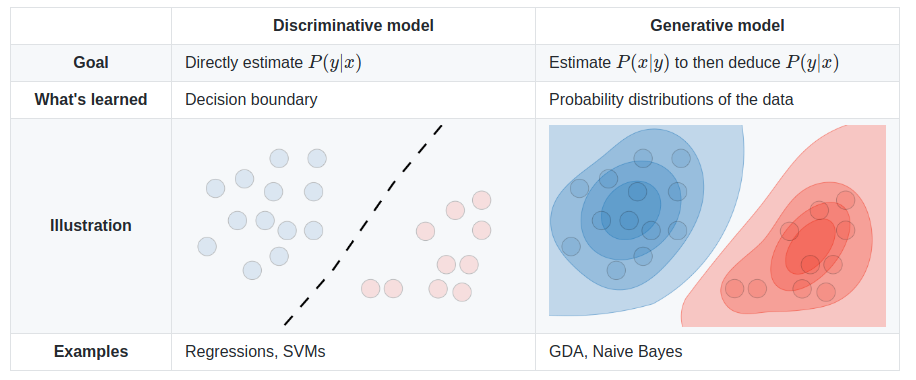
\includegraphics[width=\textwidth]{figures/4/classifiers}
	\caption{Differences between Generative and Discriminative classifiers.}
	\label{fig:classifiers}
\end{figure}

Generative Classifiers (\hyperref[eq:mle]{\emph{\Naive Bayes}}) --
\begin{itemize}
	\item Assume some functional form for \emph{conditional independence}.
	\item Estimate parameters of \data{$P(D|h)$}, \data{$P(h)$} directly from training data.
	\item Use Bayes' rule to calculate \data{$P(h|D)$}.
\end{itemize}

Why not \emph{learn} \data{$P(h | D)$} or the decision boundary \emph{directly}?
Discriminative Classifiers (\hyperref[eq:map]{\emph{Logistic Regression}}) --
\begin{itemize}
	\item Assume some functional form for \data{$P(h | D)$} or for the decision boundary.
	\item \emph{Estimate parameters} of \data{$P(h | D)$} \emph{directly} from training data.
\end{itemize}

\section{Learning a Logistic Regression Classifier}\label{sec:learning-a-logisitc-regression-classifier}
Given \data{$n$} \emph{input-output} pairs --
\begin{enumerate}
	\item A feature representation of the \emph{input}.
	For each \emph{input observation} \data{$x_{i}$}, a vector of \emph{features} \data{$[x_{1}, x_{2}, \dots, x_{d}]$}.
	\item A \emph{classification function} that computes \data{$y$}, the estimated class, via \data{$P(y|x)$}, using the \emph{sigmoid of softmax} functions.
	\item An objective function for learning, like \emph{cross-entropy loss}.
	\item An algorithm for optimizing the objective function, like \emph{stochastic gradient ascent/descent}.
\end{enumerate}

\section{Logistic Regression}\label{sec:logistic-regression}
Logistic Regression \emph{assumes} the following function form for \data{$P(y|x)$}:
\data{\[ P(y=1|x) = \frac{1}{1+e^{-\left( \sum_{i}w_{i}x_{i} + b \right)}} \]}
\begin{equation*}
\begin{aligned}[eqpurple]
	P(y=1|x) &= \frac{1}{1+e^{-\left( \sum_{i}w_{i}x_{i} + b \right)}}\\
			 &= \frac{e^{\left( \sum_{i}w_{i}x_{i} + b \right)}}{e^{\left( \sum_{i}w_{i}x_{i} + b \right)} + 1}\\
	P(y=0|x) &= 1 - \frac{1}{1+e^{\left( \sum_{i}w_{i}x_{i} + b \right)}}\\
			 &= \frac{1}{e^{\left( \sum_{i}w_{i}x_{i} + b \right)} + 1}\\
	\frac{P(y=1|x)}{P(y=0|x)} &= e^{\left( \sum_{i}w_{i}x_{i} + b \right)} > 1\\
	&\Rightarrow \sum_{i} w_{i}x_{i} + b > 0
\end{aligned}
\end{equation*}
Logistic Regression is a \emph{linear} classifier.
Turning a probability into a classifier using the \emph{logistic function}:
\[ \data{ y_{LR}\left\{ \begin{array}{clr}
	1 & \mbox{ if } P(y=1|x) \geq 0.5 & \textcolor{black}{\leftarrow w_{i}x_{i} + b \geq 0}\\
	0 & \mbox{otherwise} & \textcolor{black}{\leftarrow w_{i}x_{i} + b < 0}
\end{array} \right. } \]

\section{LR Example}\label{sec:lr-example}
Suppose we are doing \emph{binary sentiment classification} on movie review text, and we would like to know whether to assign the sentiment class \emph{position = 1} or \emph{negative = 0} to the following review:\\

It's hokey.
There are virtually no surprises, and the writing is second-rate.
So why was is so enjoyable?
For one thing, the case is great.
Another nice touch is the music.
I was overcome with the urge to get off the couch and start dancing.
It sucked me in, and it'll do the same to you.

\begin{figure}[H]
	\centering
	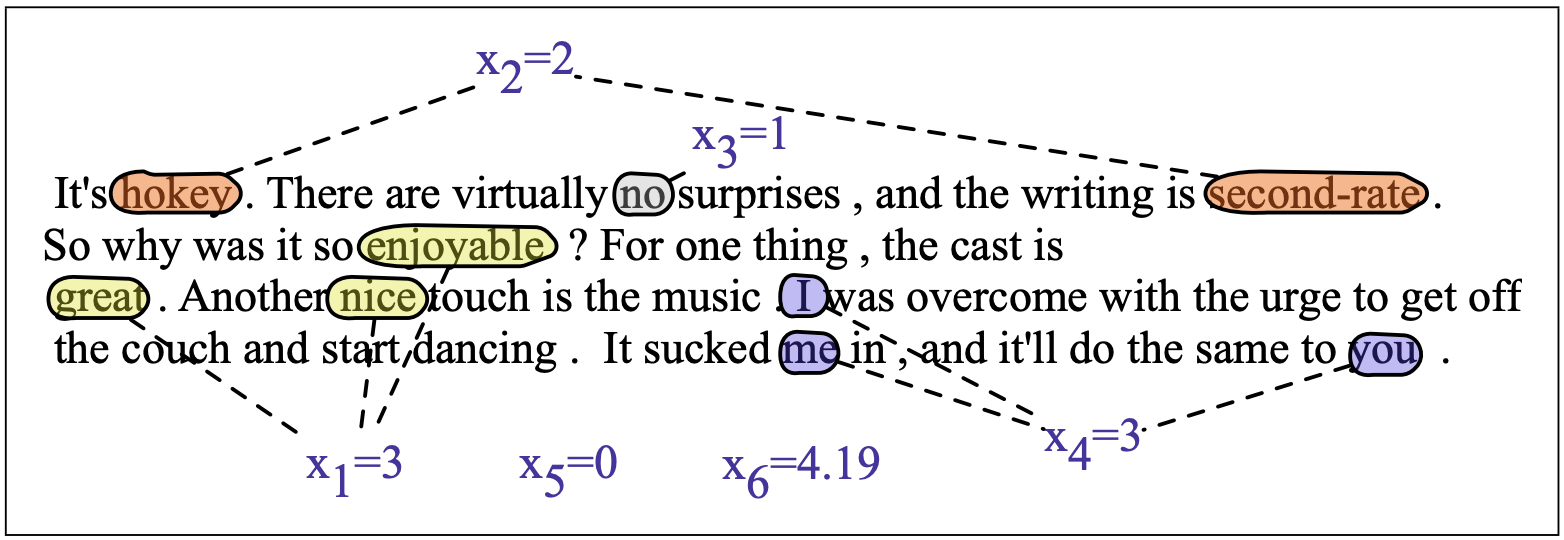
\includegraphics[width=\textwidth]{figures/4/lr_example}
	\caption{LR Example.}
	\label{fig:lr_example}
\end{figure}

\begin{figure}[H]
	\centering
	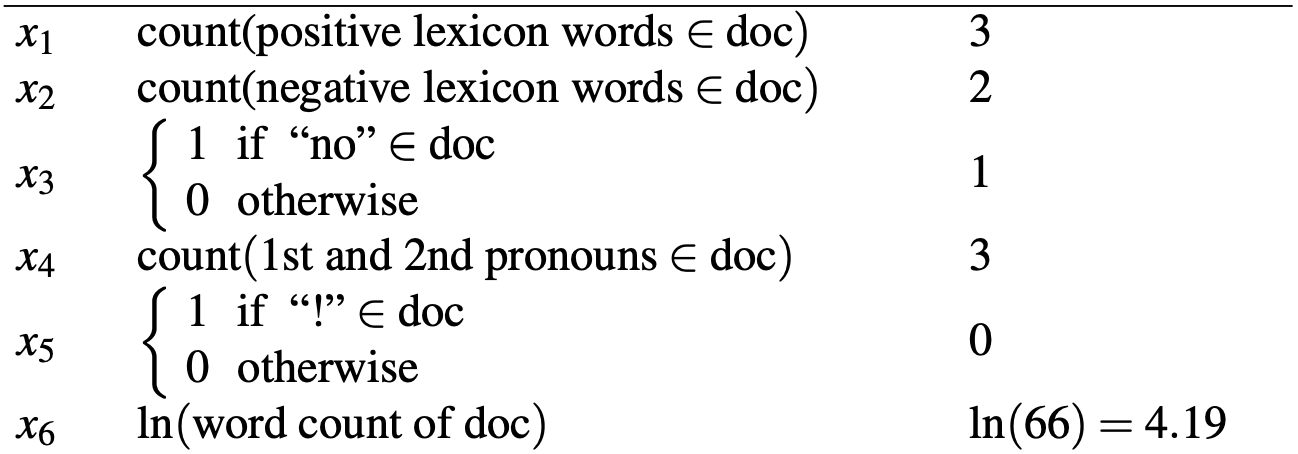
\includegraphics[width=\textwidth]{figures/4/lr_feature_vector}
	\caption{Feature vector for the LR Example.}
	\label{fig:lr_feature_vector}
\end{figure}


\section{Sentiment Classification}\label{sec:sentiment-classification}
Let's assume for the moment that we've already \emph{learned} a \emph{real-valued weight} for each of these features, and that the \emph{6 weights} corresponding to the \emph{6 features} are \data{$[2.5, -5.0, -1.2, 0.5, 2.0, 0.7]$}, while \data{$b=0.1$}.

\begin{equation*}
\begin{aligned}[eqpurple]
	P(+ve | x) &= P(y = 1 | x)\\
	&= \frac{1}{1 + e^{\left( \sum_{i} w_{i}x_{i} + b \right)}}\\
	&= \frac{1}{1 + e^{-\left( 2.5(3) + (-5)(2) + (-1.2)(1) + 0.5(3) + 2.0(0) + 0.7(4.19) + 0.1 \right)}}\\
	&= 0.30\\
	P(-ve | x) &= P(y = 0 | x)\\
	&= 1 - P(y = 1 | x)\\
	&= 1 - 0.70\\
	&= 0.30
\end{aligned}
\end{equation*}
Since \data{$P(+ve|x) > P(-ve|x)$}, the output sentiment class is \emph{positive}.

\section{Training Logistic Regression}\label{sec:training-logistic-regression}
We'll focus on \emph{binary classification}.
We \emph{parameterize} \data{$(w_{i}, b)$} as \data{$\theta$}:
\begin{equation*}
\begin{aligned}[eqpurple]
	P(y_{i} = 0|x_{i},\theta) = \frac{1}{e^{\sum_{i} w_{i}x_{i} + b}+1}\\
	P(y_{i} = 1|x_{i},\theta) = \frac{e^{\sum_{i} w_{i}x_{i} + b}}{e^{\sum_{i} w_{i}x_{i} + b}+1}\\
	P(y_{i}|x_{i},\theta) = \frac{e^{y_{i}\sum_{i} w_{i}x_{i} + b}}{e^{\sum_{i} w_{i}x_{i} + b}+1}
\end{aligned}
\end{equation*}
How do we \emph{learn parameters} \data{$\theta$}?

\section{Cross-Entropy Loss}\label{sec:cross-entropy-loss}
\begin{itemize}
	\item We want to know \emph{how far} is the \emph{classifier output} \data{$\hat{y}$} from the \emph{true output} \data{$y$}.
	Let's call this difference \data{$L(\hat{y},y)$}.
	\item Since there are only \emph{2 discrete outcomes} (0 or 1), we can express the probability \data{$P(y|x)$} from our classifiers as:
	\data{\[ P(y|x) = \hat{y}^{y}\cdot (1-\hat{y})^{1-y} \]}
	\item Goal: \emph{maximize the probability} of the correct label \data{$P(y|x)$.}
	\item Maximize:
	\data{\begin{equation*}
	\begin{aligned}
		P(y|x) &= \hat{y}^{y}\cdot (1-\hat{y})^{1-y}\\
		\log(P(y|x)) &= \log\left( \hat{y}^{y}\cdot (1-\hat{y})^{1-y} \right)\\
					 &= y\log(\hat{y})+ (1-y)\log(1-\hat{y})\\
	\end{aligned}
	\end{equation*}}
	\item We want to \emph{minimize} the \emph{cross-entropy loss}:
	\begin{equation*}
	\begin{aligned}[eqpurple]
		\mathbf{Minimize:\ } L_{CE}(\hat{y}, y) &= -\log P(y|x)\\
		&= -\left[ y\log(\hat{y}) + (1 - y)\log(1 - \hat{y}) \right]\\
		\min_{\theta} L_{CE}(\hat{y}, y) &= -\left[ y\log(\hat{y}) + (1 - y)\log(1 - \hat{y}) \right]\\
		&= -\left[ y\log\left( \frac{e^{\sum_{i} w_{i}x_{i} + b}}{1 + e^{\sum_{i} w_{i}x_{i} + b}} \right) + (1 - y)\log\left(1 - \frac{e^{\sum_{i} w_{i}x_{i} + b}}{1 + e^{\sum_{i} w_{i}x_{i} + b}}\right) \right]\\
		&= -\left[ y\left( \sum_{i} w_{i}x_{i} + b - \log\left( 1 + e^{\sum_{i} w_{i}x_{i} + b} \right) \right) + (1-y)\left( -\log\left( 1 + e^{\sum_{i} w_{i}x_{i} + b} \right) \right) \right]\\
		&= -\left[ y\left( \sum_{i} w_{i}x_{i} + b \right) - \log\left( 1 + e^{\sum_{i} w_{i}x_{i} + b} \right) \right]\\
		&= \log\left( 1 + e^{\sum_{i} w_{i}x_{i} + b} \right) + y\left( \sum_{i} w_{i}x_{i} + b \right)\\
	\end{aligned}
	\end{equation*}
\end{itemize}

\section{Minimizing Cross-Entropy Loss}\label{sec:minimizing-cross-entropy-loss}
\data{\[ \min_{\theta} L_{CE}(\hat{y}, y) \]}
\begin{itemize}
	\item Minimizing loss function \data{$L_{CE}(\hat{y},y)$} is a \emph{convex optimization problem}.
	\item \emph{Convex} functions have a \emph{global minimum}.
	\item \emph{Concave} functions have a \emph{global maxima}.
\end{itemize}

\begin{figure}[H]
	\centering
	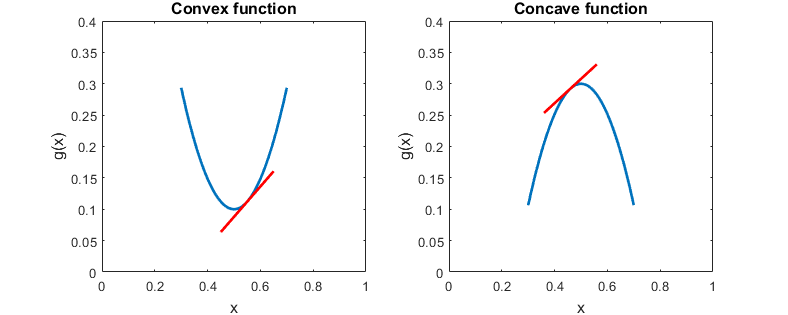
\includegraphics[width=\textwidth]{figures/4/concave_convex}
	\caption{An example of a convec and concave function.}
	\label{fig:concave-convex}
\end{figure}


\section{Optimizing a Convex/Concave Function}\label{sec:optimizing-a-convex/concave-function}
\begin{itemize}
	\item Maximum of a \emph{concave} function is \emph{equivalent} to the \emph{minimum} of a \emph{convex} function.
	\item \emph{Gradient Ascent} is used for finding the \emph{maximum} of a \emph{concave} function.
	\item \emph{Gradient Descent} is used for finding the \emph{minimum} of a \emph{convex} function.
\end{itemize}

\section{Gradients}\label{sec:gradients}
\begin{itemize}
	\item The \emph{gradient} of a \emph{function} is a \emph{vector pointing} in the \emph{direction} of the \emph{greatest increase} in a function.
\end{itemize}
\begin{description}
	\item[\emph{Gradient Ascent}:] Find the gradient of the function at the current point and \emph{move} in the \emph{same direction}.
	\item[\emph{Gradient Descent}:] Find the gradient of the function at the current point and \emph{move} in the \emph{opposite direction}.
\end{description}

\section{Gradient Descent for Logistic Regression}\label{sec:gradient-descent-for-logistic-regression}
\begin{itemize}
	\item Let us represent $\hat{y}=f(x, \theta)$
	\item Gradient:
	\begin{equation}[eqpurple]
		\nabla_{\theta} L(f(x,\theta), y) = \left[ \frac{\partial L(f(x, \theta), y)}{\partial b} , \frac{\partial L(f(x, \theta), y)}{\partial w_{1}}, \frac{\partial L(f(x, \theta), y)}{\partial w_{2}}, \dots, \frac{\partial L(f(x, \theta), y)}{\partial w_{d}} \right]
		\label{eq:gradient}
	\end{equation}
	\item Update Rule:
	\begin{equation}[eqpurple]
	\begin{aligned}[eqpurple]
		\Delta\theta &= \eta\cdot\nabla_{\theta}L(f(x,\theta), y)\\
		\theta_{t+1} &= \theta_{t} - \eta\cdot\frac{\partial}{\partial (w,b)}L(f(x,\theta), y)
	\end{aligned}
	\label{eq:update-rule}
	\end{equation}
\end{itemize}
Gradient descent algorithm will \emph{iterate} until \data{$\Delta\theta < \epsilon$}.

\begin{equation*}
\begin{aligned}[eqpurple]
	L_{CE}(f(x, \theta), y) &= \log\left( 1 + e^{\sum_{i} w_{i}x_{i} + b} \right) - y\left( \sum_{i}w_{i}x_{i} + b \right)\\
	\theta_{t+1} &= \theta_{t} - \eta\cdot\frac{\partial}{\partial (w,b)}L(f(x,\theta), y)\\
				 &= \theta_{t} - \eta\cdot x_{i}\left[ \frac{e^{\sum_{i} w_{i}x_{i} + b}}{1 + e^{\sum_{i} w_{i}x_{i} + b}} - y \right]\\
				 &= \theta_{t} - \eta\cdot x_{i}\left[ \hat{P}(y = 1|x,\theta_{t}) - y \right]
\end{aligned}
\end{equation*}

\section{Learning Rate}\label{sec:learning-rate}
\begin{itemize}
	\item \data{$\eta$} is a \emph{hyperparameter}.
	\item \emph{Large} \data{$\eta$} $\Rightarrow$ Fast convergence but larger residual error.
	Also, possible oscillations.
	\item \emph{Small} \data{$\eta$} $\Rightarrow$ Slow convergence but small residual error.
\end{itemize}

% TODO: Add the Sentiment Classification Example

\section{Batch Training}\label{sec:batch-training}
\begin{itemize}
	\item Stochastic gradient descent is called \emph{stochastic} because it chooses a \emph{single random example} at a time, moving the weights to improve performance on that single example.
	\item This results in very choppy movements, so it's \emph{common} to \emph{compute} the \emph{gradient over batches} of training instances rather than a single instance.
	\item \emph{Training data: } \data{$\{ x_{i}, y_{i} \}_{i=i\dots n}$} where \data{$x_{i} = ( x_{i1},  x_{i2}, \dots,   x_{id} )$}, \data{$n$} is the total \emph{instances} in a \emph{batch} and \data{$d$} is the \emph{dimension} of an instance.
	\begin{equation}
		\theta_{t+1} = \theta_{t} - \frac{\eta}{n} \times \sum_{i=1}^{n} xij \left[ \frac{1}{1 + e^{-\theta^{T}\vec{x}}} - y_{i} \right]
		\label{eq:batch-training}
	\end{equation}
\end{itemize}

\section{Understanding the Sigmoid}\label{sec:understanding-the-sigmoid}
\begin{itemize}
	\item Large weights lead to \hyperref[sec:fitting]{\emph{overfitting}}.
	\item \emph{Penalizing} larger weights can \hyperref[subsec:resolving-overfitting]{\emph{reduce}} overfitting.
\end{itemize}

\section{Regularization}\label{sec:regularization}
\begin{itemize}
	\item Regularization is used to \emph{avoid overfitting}.
	\item The \emph{weights} for features will \emph{attempt} to perfectly \emph{fit} details of the training set, modeling even \emph{noisy data} that just accidentally correlate with the class.
	The problem is called \emph{overfitting}.
	\item A \emph{good model} should \emph{generalize well} from the training data to the \emph{unseen test set}, but a model that \emph{overfits} will have \emph{poor generalization}.
	\item To avoid overfitting, a new \emph{regularization term} \data{$R(\theta)$} is added to the loss function.
	\begin{equation}
		\min_{\theta} L_{reg}(\hat{y}, y) = -\frac{1}{n} \sum_{i=1}^{n} \left[ y\log(\hat{y}) + (1 - y)\log(1 - \hat{y}) \right] + \lambda R(\theta)
		\label{eq:regulatization}
	\end{equation}
\end{itemize}

\section{L1 Regularization}\label{sec:l1-regularization}
\begin{itemize}
	\item L1 Regularization is also called \emph{Lasso Regularization}.
	\item Uses the L1 norm (\emph{Manhattan distance}) of the weights.
	\[ \data{ R(\theta) = ||\theta||_{1} = \sum_{j=0}^{d} |\theta_{j}| } \]
\end{itemize}
\begin{equation}
	\min_{\theta} L_{reg}(\hat{y}, y) = -\frac{1}{n} \sum_{i=1}^{n} \left[ y\log(\hat{y}) + (1 - y)\log(1 - \hat{y}) \right] + \lambda\sum_{j=0}^{d}|\theta_{j}|
	\label{eq:l1-regulatization}
\end{equation}

\section{L2 Regularization}\label{sec:l2-regularization}
\begin{itemize}
	\item L2 Regularization is also called \emph{Ridge Regularization}.
	\item Uses the square of the \emph{L2 (Euclidean) norm} of the weights.
	\[ \data{ R(\theta) = ||\theta||_{2}^{2} = \sum_{j=0}^{d} \theta_{j}^{2} } \]
\end{itemize}
\begin{equation}
	\min_{\theta} L_{reg}(\hat{y}, y) = -\frac{1}{n} \sum_{i=1}^{n} \left[ y\log(\hat{y}) + (1 - y)\log(1 - \hat{y}) \right] + \lambda\sum_{j=0}^{d} \theta_{j}^{2}
	\label{eq:l2-regulatization}
\end{equation}

\section{Example -- Spam Recognition}\label{sec:example----spam-recognition}
Let us apply logistic regression on the spam email recognition problem, assuming \data{$\eta = 3.0$} and starting with \data{$\theta_{w, b} = [0, 0, 0, 0, 0, 0]$}.
\begin{table}[H]
	\centering
	\caption{}
	\label{tab:spam-data}
	\begin{tabular}{*{7}{|C{0.1\textwidth}}|}
		\hline
		\rowcolor{lightblue} & \tableheader{and} & \tableheader{vaccine} & \tableheader{the} & \tableheader{of} & \tableheader{nigeria} & \cellcolor{red} \tableheader{y}\\
		\hline
		Email \textbf{a} & 1 & 1 & 0 & 1 & 1 & 1\\
		\hline
		Email \textbf{b} & 0 & 0 & 1 & 1 & 0 & 0\\
		\hline
		Email \textbf{c} & 0 & 1 & 1 & 0 & 0 & 1\\
		\hline
		Email \textbf{d} & 1 & 0 & 0 & 1 & 0 & 0\\
		\hline
		Email \textbf{e} & 1 & 0 & 1 & 0 & 1 & 1\\
		\hline
		Email \textbf{f} & 1 & 0 & 1 & 1 & 0 & 0\\
		\hline
	\end{tabular}
\end{table}
1 entails that a word (i.e., ``and'') is present in an email (i.e.\ ``Email \textbf{a}'') and 0 entails that a word is absent in an email.

\begin{table}[H]
	\centering
	\caption{}
	\label{tab:formatted-spam-data}
	\begin{tabular}{*{8}{|c}|}
		\hline
		\rowcolor{lightblue} & $x_{0} = \textcolor{white}{1}$ & $x_{1} = $ \tableheader{and} & $x_{2} = $ \tableheader{vaccine} & $x_{3} = $ \tableheader{the} & $x_{4} = $ \tableheader{of} & $x_{5} = $ \tableheader{nigeria} & \cellcolor{red} \tableheader{y}\\
		\hline
		Email \textbf{a} & 1 & 1 & 1 & 0 & 1 & 1 & 1\\
		\hline
		Email \textbf{b} & 1 & 0 & 0 & 1 & 1 & 0 & 0\\
		\hline
		Email \textbf{c} & 1 & 0 & 1 & 1 & 0 & 0 & 1\\
		\hline
		Email \textbf{d} & 1 & 1 & 0 & 0 & 1 & 0 & 0\\
		\hline
		Email \textbf{e} & 1 & 1 & 0 & 1 & 0 & 1 & 1\\
		\hline
		Email \textbf{f} & 1 & 1 & 0 & 1 & 1 & 0 & 0\\
		\hline
	\end{tabular}
\end{table}
The column $x_{0}$ was added to account for this bias \data{$b$}.

\data{$x = [x_{0}, x_{1}, x_{2}, x_{3}, x_{4}, x_{5}]$},  \data{$\theta = [b, w_{1}, w_{2}, w_{3}, w_{4}, w_{5}]$}

\section{Training Phase}\label{sec:training-phase}
\begin{equation*}
\begin{aligned}[eqpurple]
	\theta_{t+1} = \theta_{t} - \frac{\eta}{n}\times \sum_{i=1}^{n} x_{ij}\left[ \frac{1}{1 + e^{-\theta^{T}\vec{x}}} - y_{i} \right]
\end{aligned}
\end{equation*}

\begin{enumerate}[label=\arabic*)]
	\item Calculate the factor $-\theta^{T}\vec{x}$ for every example in the dataset.
	\item Calculate the factor $\sum_{i=1}^{n} x_{ij}\left[ \frac{1}{1 + e^{-\theta^{T}\vec{x}}} - y_{i} \right]$ for every example in the dataset, for every \data{$\theta$}
	\item Compute every \data{$\theta$}
\end{enumerate}

\begin{table}[H]
	\centering
	\caption{}
	\label{tab:training-0}
	\begin{tabular}{*{4}{|c}|}
		\hline
		\textcolor{lightblue}{$x$} & \textcolor{red}{$y$} & $\theta^{T}\vec{x}$ & $\left( \frac{1}{1 + e^{-\vec{\theta}^{T}\vec{x}} } - \textcolor{red}{y} \right) \textcolor{lightblue}{x_{0}}$\\
		\hline
		[1, 1, 1, 0, 1, 1] & \textbf{1} & $[0, 0, 0, 0, 0, 0] \times [1, 1, 1, 0, 1, 1] = 0$ & $\left( \frac{1}{1 + e^{0}} - \textcolor{red}{\mathbf{1}} \right) \times \textcolor{lightblue}{1} = -0.5$\\
		\hline
		[1, 0, 0, 1, 1, 0] & \textbf{0} & $[0, 0, 0, 0, 0, 0] \times [1, 0, 0, 1, 1, 0] = 0$ & $\left( \frac{1}{1 + e^{0}} - \textcolor{red}{\mathbf{0}} \right) \times \textcolor{lightblue}{1} = 0.5$\\
		\hline
		[1, 0, 1, 1, 0, 0] & \textbf{1} & $[0, 0, 0, 0, 0, 0] \times [1, 0, 1, 1, 0, 0] = 0$ & $\left( \frac{1}{1 + e^{0}} - \textcolor{red}{\mathbf{1}} \right) \times \textcolor{lightblue}{1} = -0.5$\\
		\hline
		[1, 1, 0, 0, 1, 0] & \textbf{0} & $[0, 0, 0, 0, 0, 0] \times [1, 1, 0, 0, 1, 0] = 0$ & $\left( \frac{1}{1 + e^{0}} - \textcolor{red}{\mathbf{0}} \right) \times \textcolor{lightblue}{1} = 0.5$\\
		\hline
		[1, 1, 0, 1, 0, 1] & \textbf{1} & $[0, 0, 0, 0, 0, 0] \times [1, 1, 0, 1, 0, 1] = 0$ & $\left( \frac{1}{1 + e^{0}} - \textcolor{red}{\mathbf{1}} \right) \times \textcolor{lightblue}{1} = -0.5$\\
		\hline
		[1, 1, 0, 1, 1, 0] & \textbf{0} & $[0, 0, 0, 0, 0, 0] \times [1, 1, 0, 1, 1, 0] = 0$ & $\left( \frac{1}{1 + e^{0}} - \textcolor{red}{\mathbf{0}} \right) \times \textcolor{lightblue}{1} = 0.5$\\
		\hline
	\end{tabular}
\end{table}
\begin{equation*}
\begin{aligned}[eqpurple]
	\sum_{i=1}^6 x_{i0} \left[ \frac{1}{ 1 + e^{\vec{\theta^{T}}\vec{x}}} - y_{i} \right] &= -0.5 + 0.5 - 0.5 + 0.5 - 0.5 + 0.5 \\
&= 0.0
\end{aligned}
\end{equation*}
\begin{table}[H]
	\centering
	\caption{}
	\label{tab:training-1}
	\begin{tabular}{*{4}{|c}|}
		\hline
		\textcolor{lightblue}{$x$} & \textcolor{red}{$y$} & $\theta^{T}\vec{x}$ & $\left( \frac{1}{1 + e^{-\vec{\theta}^{T}\vec{x}} } - \textcolor{red}{y} \right) \textcolor{lightblue}{x_{1}}$\\
		\hline
		[1, 1, 1, 0, 1, 1] & \textbf{1} & $[0, 0, 0, 0, 0, 0] \times [1, 1, 1, 0, 1, 1] = 0$ & $\left( \frac{1}{1 + e^{0}} - \textcolor{red}{\mathbf{1}} \right) \times \textcolor{lightblue}{1} = -0.5$\\
		\hline
		[1, 0, 0, 1, 1, 0] & \textbf{0} & $[0, 0, 0, 0, 0, 0] \times [1, 0, 0, 1, 1, 0] = 0$ & $\left( \frac{1}{1 + e^{0}} - \textcolor{red}{\mathbf{0}} \right) \times \textcolor{lightblue}{0} = 0$\\
		\hline
		[1, 0, 1, 1, 0, 0] & \textbf{1} & $[0, 0, 0, 0, 0, 0] \times [1, 0, 1, 1, 0, 0] = 0$ & $\left( \frac{1}{1 + e^{0}} - \textcolor{red}{\mathbf{1}} \right) \times \textcolor{lightblue}{0} = 0$\\
		\hline
		[1, 1, 0, 0, 1, 0] & \textbf{0} & $[0, 0, 0, 0, 0, 0] \times [1, 1, 0, 0, 1, 0] = 0$ & $\left( \frac{1}{1 + e^{0}} - \textcolor{red}{\mathbf{0}} \right) \times \textcolor{lightblue}{1} = 0.5$\\
		\hline
		[1, 1, 0, 1, 0, 1] & \textbf{1} & $[0, 0, 0, 0, 0, 0] \times [1, 1, 0, 1, 0, 1] = 0$ & $\left( \frac{1}{1 + e^{0}} - \textcolor{red}{\mathbf{1}} \right) \times \textcolor{lightblue}{1} = -0.5$\\
		\hline
		[1, 1, 0, 1, 1, 0] & \textbf{0} & $[0, 0, 0, 0, 0, 0] \times [1, 1, 0, 1, 1, 0] = 0$ & $\left( \frac{1}{1 + e^{0}} - \textcolor{red}{\mathbf{0}} \right) \times \textcolor{lightblue}{1} = 0.5$\\
		\hline
	\end{tabular}
\end{table}
\begin{equation*}
\begin{aligned}[eqpurple]
	\sum_{i=1}^6 x_{i1} \left[ \frac{1}{ 1 + e^{\vec{\theta^{T}}\vec{x}}} - y_{i} \right] &= -0.5 + 0 + 0 + 0.5 - 0.5 + 0.5 \\
&= 0.0
\end{aligned}
\end{equation*}
\begin{table}[H]
	\centering
	\caption{}
	\label{tab:training-2}
	\begin{tabular}{*{4}{|c}|}
		\hline
		\textcolor{lightblue}{$x$} & \textcolor{red}{$y$} & $\theta^{T}\vec{x}$ & $\left( \frac{1}{1 + e^{-\vec{\theta}^{T}\vec{x}} } - \textcolor{red}{y} \right) \textcolor{lightblue}{x_{2}}$\\
		\hline
		[1, 1, 1, 0, 1, 1] & \textbf{1} & $[0, 0, 0, 0, 0, 0] \times [1, 1, 1, 0, 1, 1] = 0$ & $\left( \frac{1}{1 + e^{0}} - \textcolor{red}{\mathbf{1}} \right) \times \textcolor{lightblue}{1} = -0.5$\\
		\hline
		[1, 0, 0, 1, 1, 0] & \textbf{0} & $[0, 0, 0, 0, 0, 0] \times [1, 0, 0, 1, 1, 0] = 0$ & $\left( \frac{1}{1 + e^{0}} - \textcolor{red}{\mathbf{0}} \right) \times \textcolor{lightblue}{0} = 0$\\
		\hline
		[1, 0, 1, 1, 0, 0] & \textbf{1} & $[0, 0, 0, 0, 0, 0] \times [1, 0, 1, 1, 0, 0] = 0$ & $\left( \frac{1}{1 + e^{0}} - \textcolor{red}{\mathbf{1}} \right) \times \textcolor{lightblue}{1} = -0.5$\\
		\hline
		[1, 1, 0, 0, 1, 0] & \textbf{0} & $[0, 0, 0, 0, 0, 0] \times [1, 1, 0, 0, 1, 0] = 0$ & $\left( \frac{1}{1 + e^{0}} - \textcolor{red}{\mathbf{0}} \right) \times \textcolor{lightblue}{0} = 0$\\
		\hline
		[1, 1, 0, 1, 0, 1] & \textbf{1} & $[0, 0, 0, 0, 0, 0] \times [1, 1, 0, 1, 0, 1] = 0$ & $\left( \frac{1}{1 + e^{0}} - \textcolor{red}{\mathbf{1}} \right) \times \textcolor{lightblue}{0} = 0$\\
		\hline
		[1, 1, 0, 1, 1, 0] & \textbf{0} & $[0, 0, 0, 0, 0, 0] \times [1, 1, 0, 1, 1, 0] = 0$ & $\left( \frac{1}{1 + e^{0}} - \textcolor{red}{\mathbf{0}} \right) \times \textcolor{lightblue}{0} = 0$\\
		\hline
	\end{tabular}
\end{table}
\begin{equation*}
\begin{aligned}[eqpurple]
	\sum_{i=1}^6 x_{i2} \left[ \frac{1}{ 1 + e^{\vec{\theta^{T}}\vec{x}}} - y_{i} \right] &= -0.5 + 0 - 0.5 + 0 + 0 + 0 \\
&= -1.0
\end{aligned}
\end{equation*}
\begin{table}[H]
	\centering
	\caption{}
	\label{tab:training-3}
	\begin{tabular}{*{4}{|c}|}
		\hline
		\textcolor{lightblue}{$x$} & \textcolor{red}{$y$} & $\theta^{T}\vec{x}$ & $\left( \frac{1}{1 + e^{-\vec{\theta}^{T}\vec{x}} } - \textcolor{red}{y} \right) \textcolor{lightblue}{x_{3}}$\\
		\hline
		[1, 1, 1, 0, 1, 1] & \textbf{1} & $[0, 0, 0, 0, 0, 0] \times [1, 1, 1, 0, 1, 1] = 0$ & $\left( \frac{1}{1 + e^{0}} - \textcolor{red}{\mathbf{1}} \right) \times \textcolor{lightblue}{0} = 0$\\
		\hline
		[1, 0, 0, 1, 1, 0] & \textbf{0} & $[0, 0, 0, 0, 0, 0] \times [1, 0, 0, 1, 1, 0] = 0$ & $\left( \frac{1}{1 + e^{0}} - \textcolor{red}{\mathbf{0}} \right) \times \textcolor{lightblue}{1} = 0.5$\\
		\hline
		[1, 0, 1, 1, 0, 0] & \textbf{1} & $[0, 0, 0, 0, 0, 0] \times [1, 0, 1, 1, 0, 0] = 0$ & $\left( \frac{1}{1 + e^{0}} - \textcolor{red}{\mathbf{1}} \right) \times \textcolor{lightblue}{1} = -0.5$\\
		\hline
		[1, 1, 0, 0, 1, 0] & \textbf{0} & $[0, 0, 0, 0, 0, 0] \times [1, 1, 0, 0, 1, 0] = 0$ & $\left( \frac{1}{1 + e^{0}} - \textcolor{red}{\mathbf{0}} \right) \times \textcolor{lightblue}{0} = 0$\\
		\hline
		[1, 1, 0, 1, 0, 1] & \textbf{1} & $[0, 0, 0, 0, 0, 0] \times [1, 1, 0, 1, 0, 1] = 0$ & $\left( \frac{1}{1 + e^{0}} - \textcolor{red}{\mathbf{1}} \right) \times \textcolor{lightblue}{1} = -0.5$\\
		\hline
		[1, 1, 0, 1, 1, 0] & \textbf{0} & $[0, 0, 0, 0, 0, 0] \times [1, 1, 0, 1, 1, 0] = 0$ & $\left( \frac{1}{1 + e^{0}} - \textcolor{red}{\mathbf{0}} \right) \times \textcolor{lightblue}{1} = 0.5$\\
		\hline
	\end{tabular}
\end{table}
\begin{equation*}
\begin{aligned}[eqpurple]
	\sum_{i=1}^6 x_{i3} \left[ \frac{1}{ 1 + e^{\vec{\theta^{T}}\vec{x}}} - y_{i} \right] &= 0 + 0.5 - 0.5 + 0 - 0.5 + 0.5 \\
&= 0.0
\end{aligned}
\end{equation*}
\begin{table}[H]
	\centering
	\caption{}
	\label{tab:training-4}
	\begin{tabular}{*{4}{|c}|}
		\hline
		\textcolor{lightblue}{$x$} & \textcolor{red}{$y$} & $\theta^{T}\vec{x}$ & $\left( \frac{1}{1 + e^{-\vec{\theta}^{T}\vec{x}} } - \textcolor{red}{y} \right) \textcolor{lightblue}{x_{4}}$\\
		\hline
		[1, 1, 1, 0, 1, 1] & \textbf{1} & $[0, 0, 0, 0, 0, 0] \times [1, 1, 1, 0, 1, 1] = 0$ & $\left( \frac{1}{1 + e^{0}} - \textcolor{red}{\mathbf{1}} \right) \times \textcolor{lightblue}{1} = -0.5$\\
		\hline
		[1, 0, 0, 1, 1, 0] & \textbf{0} & $[0, 0, 0, 0, 0, 0] \times [1, 0, 0, 1, 1, 0] = 0$ & $\left( \frac{1}{1 + e^{0}} - \textcolor{red}{\mathbf{0}} \right) \times \textcolor{lightblue}{1} = 0.5$\\
		\hline
		[1, 0, 1, 1, 0, 0] & \textbf{1} & $[0, 0, 0, 0, 0, 0] \times [1, 0, 1, 1, 0, 0] = 0$ & $\left( \frac{1}{1 + e^{0}} - \textcolor{red}{\mathbf{1}} \right) \times \textcolor{lightblue}{0} = 0$\\
		\hline
		[1, 1, 0, 0, 1, 0] & \textbf{0} & $[0, 0, 0, 0, 0, 0] \times [1, 1, 0, 0, 1, 0] = 0$ & $\left( \frac{1}{1 + e^{0}} - \textcolor{red}{\mathbf{0}} \right) \times \textcolor{lightblue}{1} = 0.5$\\
		\hline
		[1, 1, 0, 1, 0, 1] & \textbf{1} & $[0, 0, 0, 0, 0, 0] \times [1, 1, 0, 1, 0, 1] = 0$ & $\left( \frac{1}{1 + e^{0}} - \textcolor{red}{\mathbf{1}} \right) \times \textcolor{lightblue}{0} = 0$\\
		\hline
		[1, 1, 0, 1, 1, 0] & \textbf{0} & $[0, 0, 0, 0, 0, 0] \times [1, 1, 0, 1, 1, 0] = 0$ & $\left( \frac{1}{1 + e^{0}} - \textcolor{red}{\mathbf{0}} \right) \times \textcolor{lightblue}{1} = 0.5$\\
		\hline
	\end{tabular}
\end{table}
\begin{equation*}
\begin{aligned}[eqpurple]
	\sum_{i=1}^6 x_{i4} \left[ \frac{1}{ 1 + e^{\vec{\theta^{T}}\vec{x}}} - y_{i} \right] &= -0.5 + 0.5 + 0 + 0.5 + 0 + 0.5 \\
&= 1.0
\end{aligned}
\end{equation*}
\begin{table}[H]
	\centering
	\caption{}
	\label{tab:training-5}
	\begin{tabular}{*{4}{|c}|}
		\hline
		\textcolor{lightblue}{$x$} & \textcolor{red}{$y$} & $\theta^{T}\vec{x}$ & $\left( \frac{1}{1 + e^{-\vec{\theta}^{T}\vec{x}} } - \textcolor{red}{y} \right) \textcolor{lightblue}{x_{5}}$\\
		\hline
		[1, 1, 1, 0, 1, 1] & \textbf{1} & $[0, 0, 0, 0, 0, 0] \times [1, 1, 1, 0, 1, 1] = 0$ & $\left( \frac{1}{1 + e^{0}} - \textcolor{red}{\mathbf{1}} \right) \times \textcolor{lightblue}{1} = -0.5$\\
		\hline
		[1, 0, 0, 1, 1, 0] & \textbf{0} & $[0, 0, 0, 0, 0, 0] \times [1, 0, 0, 1, 1, 0] = 0$ & $\left( \frac{1}{1 + e^{0}} - \textcolor{red}{\mathbf{0}} \right) \times \textcolor{lightblue}{0} = 0$\\
		\hline
		[1, 0, 1, 1, 0, 0] & \textbf{1} & $[0, 0, 0, 0, 0, 0] \times [1, 0, 1, 1, 0, 0] = 0$ & $\left( \frac{1}{1 + e^{0}} - \textcolor{red}{\mathbf{1}} \right) \times \textcolor{lightblue}{0} = 0$\\
		\hline
		[1, 1, 0, 0, 1, 0] & \textbf{0} & $[0, 0, 0, 0, 0, 0] \times [1, 1, 0, 0, 1, 0] = 0$ & $\left( \frac{1}{1 + e^{0}} - \textcolor{red}{\mathbf{0}} \right) \times \textcolor{lightblue}{0} = 0$\\
		\hline
		[1, 1, 0, 1, 0, 1] & \textbf{1} & $[0, 0, 0, 0, 0, 0] \times [1, 1, 0, 1, 0, 1] = 0$ & $\left( \frac{1}{1 + e^{0}} - \textcolor{red}{\mathbf{1}} \right) \times \textcolor{lightblue}{1} = -0.5$\\
		\hline
		[1, 1, 0, 1, 1, 0] & \textbf{0} & $[0, 0, 0, 0, 0, 0] \times [1, 1, 0, 1, 1, 0] = 0$ & $\left( \frac{1}{1 + e^{0}} - \textcolor{red}{\mathbf{0}} \right) \times \textcolor{lightblue}{0} = 0$\\
		\hline
	\end{tabular}
\end{table}
\begin{equation*}
\begin{aligned}[eqpurple]
	\sum_{i=1}^6 x_{i5} \left[ \frac{1}{ 1 + e^{\vec{\theta^{T}}\vec{x}}} - y_{i} \right] &= -0.5 + 0 + 0 + 0 - 0.5 + 0 \\
&= -1.0
\end{aligned}
\end{equation*}


\begin{equation*}
\begin{aligned}
	\theta_{1} &= \theta_{0} - \frac{\eta}{n} \times \sum_{i=1}^{n} x_{ij} \left[ \frac{1}{1 + e^{-\theta^{T}x}} - y_{i} \right]\\
				&= \left[ \begin{array}{c}
					0\\
					0\\
					0\\
					0\\
					0\\
					0\\
			    \end{array} \right] - \frac{3}{6}\left[ \begin{array}{c}
					0\\
					0\\
					-1\\
					0\\
					1\\
					-1\\
			    \end{array} \right]\\
				&= \left[ \begin{array}{c}
					0\\
					0\\
					0\\
					0\\
					0\\
					0\\
			   \end{array} \right] - \frac{1}{2}\left[ \begin{array}{c}
					0\\
					0\\
					-1\\
					0\\
					1\\
					-1\\
			   \end{array} \right]\\
				&= \left[ \begin{array}{c}
					0\\
					0\\
					\frac{1}{2}\\
					0\\
					-\frac{1}{2}\\
					\frac{1}{2}\\
			   \end{array} \right]\\
\end{aligned}
\end{equation*}

\section{Testing Phase}\label{sec:testing-phase}
Let us test logistic regression on the spam email recognition problem using the \data{$\theta = [0, 0, 0.5, 0, -0.5, 0.5]$}.
\begin{table}[H]
	\centering
	\caption{}
	\label{tab:training-5}
	\begin{tabular}{*{5}{|c}|}
		\hline
		\textcolor{lightblue}{$x$} & \textcolor{red}{$y$} & $\theta^{T}\vec{x}$ & $\mathbf{P} = \left( \frac{1}{1 + e^{-\vec{\theta}^{T}\vec{x}} } - y \right) $ & \textcolor{red}{\textbf{Predicted Class} $\hat{y}$}\\
		\hline
		[1, 1, 1, 0, 1, 1] & \textbf{1} & $[0, 0, 0.5, 0, -0.5, 0.5] \times [1, 1, 1, 0, 1, 1] = 0.5$ & 0.622459331 & \textbf{1} \\
		\hline
		[1, 0, 0, 1, 1, 0] & \textbf{0} & $[0, 0, 0.5, 0, -0.5, 0.5] \times [1, 0, 0, 1, 1, 0] = -0.5$ & 0.377540669 & \textbf{0} \\
		\hline
		[1, 0, 1, 1, 0, 0] & \textbf{1} & $[0, 0, 0.5, 0, -0.5, 0.5] \times [1, 0, 1, 1, 0, 0] = 0.5$ & 0.622459331 & \textbf{1} \\
		\hline
		[1, 1, 0, 0, 1, 0] & \textbf{0} & $[0, 0, 0.5, 0, -0.5, 0.5] \times [1, 1, 0, 0, 1, 0] = -0.5$ & 0.377540669 & \textbf{0} \\
		\hline
		[1, 1, 0, 1, 0, 1] & \textbf{1} & $[0, 0, 0.5, 0, -0.5, 0.5] \times [1, 1, 0, 1, 0, 1] = 0.5$ & 0.622459331 & \textbf{1} \\
		\hline
		[1, 1, 0, 1, 1, 0] & \textbf{0} & $[0, 0, 0.5, 0, -0.5, 0.5] \times [1, 1, 0, 1, 1, 0] = -0.5$ & 0.377540669 & \textbf{0} \\
		\hline
	\end{tabular}
\end{table}

No Misclassification

\section{Multinomial Logistic Regression}\label{sec:multinomial-logistic-regression}
\begin{itemize}
	\item The \emph{loss function} for multinomial logistic regression \emph{generalizes} the loss function for binary logistic regression from \data{$2$} to \data{$K$} \emph{classes}.
	\item The \emph{true label} \data{$y$} is a vector with \data{$K$} elements, each corresponding to a class, with \data{$y_{c} = 1$} if the \emph{correct class} is \data{$c$}, with all \emph{other elements} of \data{$y$} being \data{$0$}.
	\item The \emph{classifier} will produce an \emph{estimate vector} with \data{$K$} elements \data{$\hat{y}$}, each element \data{$\hat{y}_{k}$} of which represents the estimated \emph{probability} \data{$P(y_{k} = 1 | x)$}.
\end{itemize}

\begin{gather}
	\Call{Softmax}{z_{i}} = \frac{\exp(z_{i})}{\sum_{j=1}^{K} \exp{z_{j}}}\ \ 1 \leq i \leq K\\
	\label{eq:multinomial-softmax}
	%
	L_{CE}(\hat{y}, y) = -\sum_{k=1}^{K} y_{k} \log(\hat{y}_{k}) \\
	\begin{aligned}
		L_{CE}(\hat{y}, y) &= -\log(\hat{y}_{c})\\
						   &= -\log\left( \frac{e^{\sum_{i=1}^{d} w_{c}x_{i} + b_{c}}}{\sum_{j=1}^{K} e^{\sum_{i=1}^{d} w_{j}x_{i} + b_{j}}} \right)
	\end{aligned}\\
	\label{eq:multinomial-loss}
	\frac{\partial L_{CE}}{\partial (w_{k}, b_{k})} = x_{i}\left[ \frac{e^{\sum_{i=1}^{d} w_{k}x_{i} + b_{k}}}{\sum_{j=1}^{K} e^{\sum_{i=1}^{d} w_{j}x_{i} + b_{j}}} - y_{k} \right]
\end{gather}

\section{Conclusion}\label{sec:conclusion-4}
Logistic Regression --
\begin{itemize}
	\item is a discriminative classifier,
	\item is a linear classifier,
	\item optimizes by minimizing the cross-entropy loss via gradient descent,
	\item trains parameters:
	\begin{itemize}
		\item begins with initial weight vector,
		\item modifies it iteratively to minimize the loss function.
	\end{itemize}
\end{itemize}

\end{document}
